\chapter{Pianificazione}\label{Pianificazione}
\begin{flushleft}
Lo sviluppo del\glossario{progetto}è diviso in cinque periodi:
\begin{itemize}
    \item \textbf{Analisi} (AN);
    \item \textbf{Revisione Analisi} (RA);
    \item \textbf{Progettazione della base tecnologica} (PT);
    \item \textbf{Progettazione di Dettaglio e Codifica} (PDC);
    \item \textbf{Validazione} (VV).
\end{itemize}
In ogni periodo sono presenti delle attività da svolgere, alle quali sono associate una o più risorse. Ogni attività è sottoposta a \textit{verifica$_{G}$}, per semplificare il processo di Validazione. Il \textit{Responsabile} è tenuto a rendere più dettagliata la pianificazione delle attività.\\
Le attività sono suddivise in più sotto-attività.\\
Nel\glossario{Gantt}vengono riportate:
\begin{itemize}
    \item \textbf{Attività:} contengono più sotto-attività. Nel Gantt sono rappresentate con una linea grigia;
    \item \textbf{Milestone$_{G}$:} rappresenta la data ultima prevista per il completamento di un insieme prestabilito di attività. Ha durata di 0 (zero) giorni e coincide con la data della successiva revisione o l'approvazione complessiva di tali attività. È rappresentata nel Gantt con un rombo giallo;
    \item \textbf{Sotto-attività:} attività atomiche che possono essere svolte da una persona. Nel Gantt sono rappresentate con una linea blu.  
\end{itemize}
\section{Analisi}\label{Analisi}
\textbf{Periodo:} da 2018-11-16 a 2019-01-14\\L'Analisi inizia in concomitanza con la pubblicazione dei\glossario{capitolati}d’appalto e termina alla prima settimana della  Revisione dei Requisiti (RR).\\
In questo periodo vengono scritti i seguenti documenti:
\begin{itemize}
    \item \textbf{Studio di Fattibilità:} vengono valutati tutti i capitolati d'appalto. La valutazione è basata sull'interesse personale di ogni membro del gruppo, sulla complessità prevista e sui rischi che possono emergere. Viene data anche una descrizione generale del capitolato e una analisi preliminare.\\Viene svolta come prima attività, in quanto ritenuta bloccante per l'\textit{Analisi dei requisiti};
    \item \textbf{Norme di Progetto:} le \textit{Norme di Progetto} contengono le regole che il gruppo dovrà seguire durante l'attuazione di tutte le attività. I verificatori certificheranno il rispetto delle norme;
    \item \textbf{Analisi dei Requisiti:} l'analisi preliminare dello \textit{Studio di Fattibilità} viene approfondita.
    In questo documento vengono definiti i requisiti che il prodotto dovrà soddisfare;
    \item \textbf{Piano di Progetto:} il \textit{Responsabile} redige il \textit{Piano di Progetto}, rispettando i vincoli posti dalla \textit{proponente$_{G}$}.\\Questo documento ha l'obiettivo di regolare le attività svolte dal gruppo;
    \item \textbf{Piano di Qualifica:} il \textit{Piano di Qualifica} contiene le strategie utili al raggiungimento degli obiettivi della \textit{proponente$_{G}$}, del gruppo e inerenti alla qualità dei processi di sviluppo.\\L'obiettivo è rendere la qualità quantificabile e misurabile;
    \item \textbf{Glossario:} scritto in modo incrementale, contiene la spiegazione dei termini più tecnici utilizzati nei documenti. Questa attività è svolta da tutti i membri del gruppo, in parallelo con la redazione di tutti i documenti;
    \item \textbf{Lettera di presentazione:} documento presentato al committente che permette al gruppo di partecipare alla gara d’appalto per il \textit{capitolato$_{G}$}.
\end{itemize}
I ruoli maggiormente coinvolti sono: \textit{Responsabile}, \textit{Amministratore} e \textit{Analista}.
\begin{figure} [h]
    \centering
    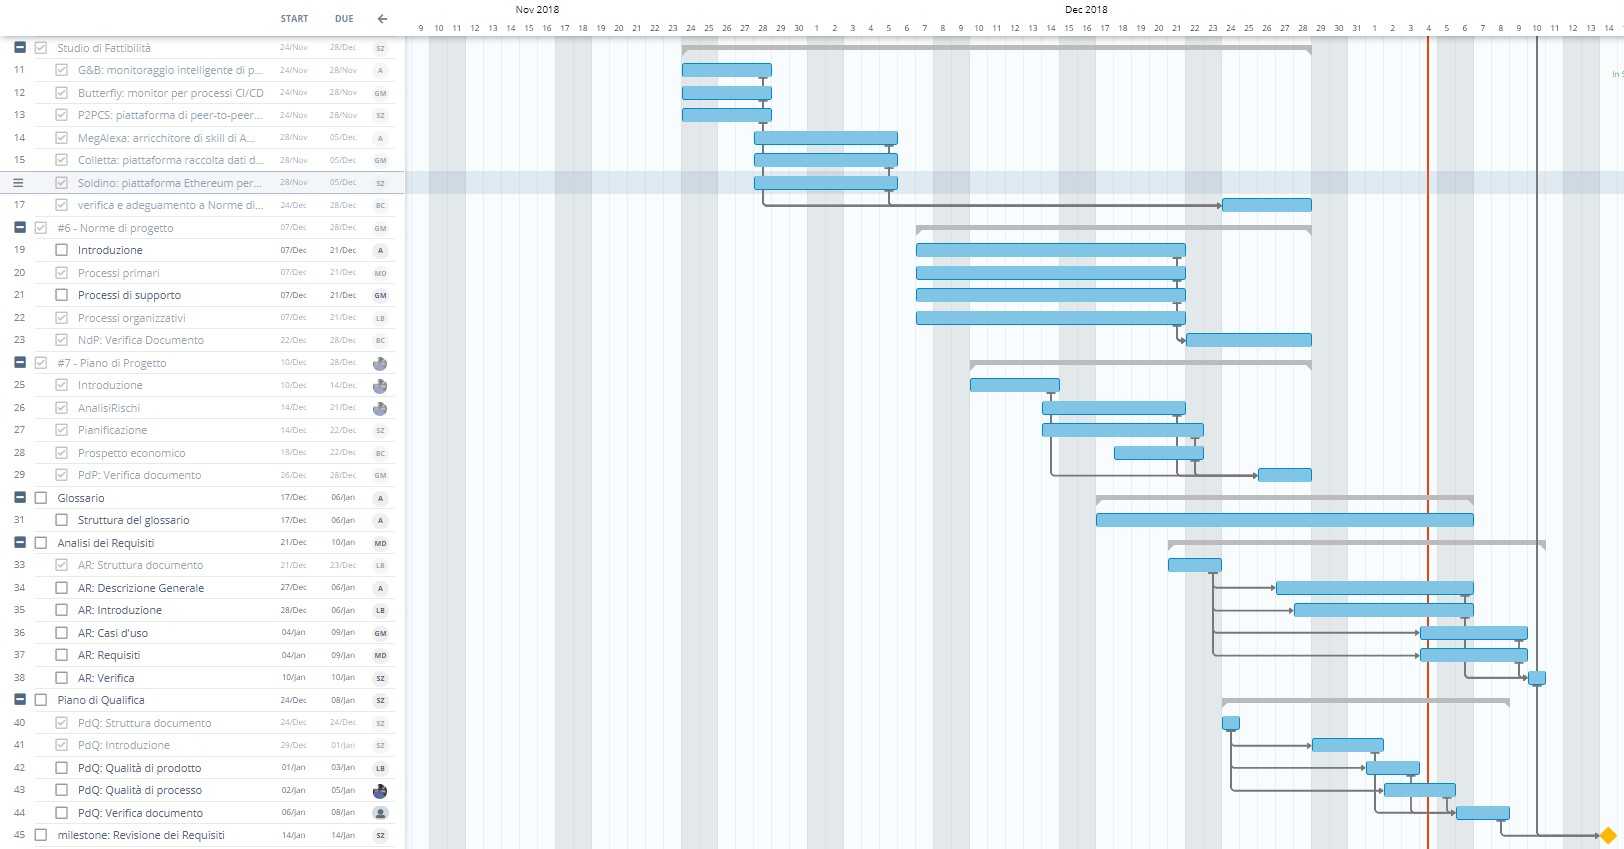
\includegraphics[scale=0.3]{./images/analisi.jpg}
    \caption{\textit{Diagramma di Gantt$_{G}$}: Analisi}\label{G1}
\end{figure}
\section{Revisione Analisi}
\textbf{Periodo:} da 2019-01-21 a 2019-02-07\\
La Revisione Analisi inizia dopo la Revisione dei Requisiti e termina con l’inizio della Progettazione della base tecnologica. Questo periodo viene utilizzato dal team per consolidare i requisiti richiesti dal sistema e per migliorare i documenti già redatti.\\
Le attività della periodo di Revisione Analisi sono:
\begin{itemize}
    \item \textbf{Incremento e Verifica$_{G}$:} tutti i documenti vengono aggiornati in base ai risultati della Revisione dei Requisiti;
    \item \textbf{Glossario:} questa attività consiste nel miglioramento del \textit{Glossario};
    \item \textbf{Consolidamento Requisiti:} correzione e possibile modifica di alcuni requisiti;
    \item \textbf{Studio tecnologie per la progettazione:} il gruppo studia quali tecnologie verranno utilizzate durante lo sviluppo del \textit{Proof of concept$_{G}$}.  
\end{itemize}
I ruoli maggiormente coinvolti sono: \textit{Responsabile}, \textit{Verificatore} e \textit{Analista}.
\begin{figure} [h]
    \centering
    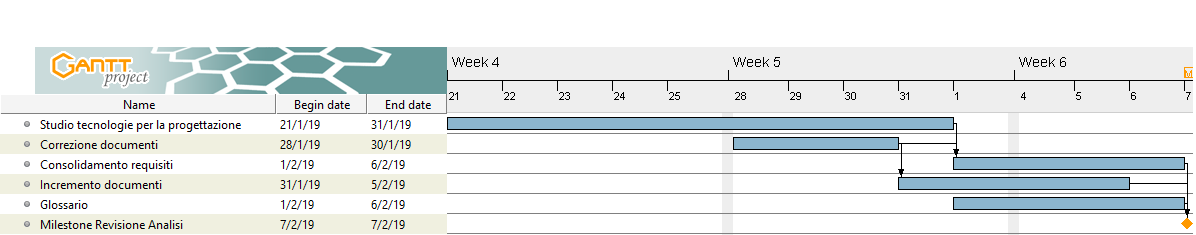
\includegraphics[scale=0.45]{./images/ZeroSevenGanttRevisioneA.png}
    \caption{\textit{Diagramma di Gantt$_{G}$}: Revisione Analisi }\label{G2}
\end{figure}
\newpage
\section{Progettazione della base tecnologica}
\textbf{Periodo:} da 2019-02-07 a 2019-03-08\\
La Progettazione della base tecnologica inizia al termine della Revisione Analisi e qui dovrà essere creato un prototipo del\glossario{prodotto}finale che verrà presentato al termine di tale periodo nella Revisione di Progettazione.\\
Le attività della periodo di Progettazione della base tecnologica sono:
\begin{itemize}
	\item \textbf{Correzione e incremento documenti};
	\item \textbf{Sviluppo Android }: Vengono studiate, progettate in dettaglio e implementate le componenti che fanno parte del \textit{Proof of}\glossario{concept}lato Applicazione Android; 
	\item \textbf{Sviluppo skill}: Vengono studiate, progettate in dettaglio e implementate le componenti che fanno parte del Proof of concept lato Skill; 
    \item\textbf{Impostazione ambiente AWS}: vengono studiate e integrate per il \textit{Proof of concept$_{G}$} le componenti \textit{AWS$_{G}$}: \textit{AWS Lambda$_{G}$}, \textit{API}\glossario{Gateway}e \textit{DynamoDB$_{G}$};
    \item \textbf{Presentazione technology baseline:} viene presentata in video call (VC) la technology baseline. Questa presentazione è una milestone che richiede il completamento del Proof of concept;
    \item \textbf{Adeguamento \textbf{Proof of concept$_{G}$} in seguito alla VC}.
\end{itemize}
I ruoli maggiormente coinvolti sono: \textit{Responsabile}, \textit{Amministratore}, \textit{Progettista}, \textit{Programmatore}, \textit{Verificatore} e \textit{Analista}.
\begin{figure} [h]
    \centering
    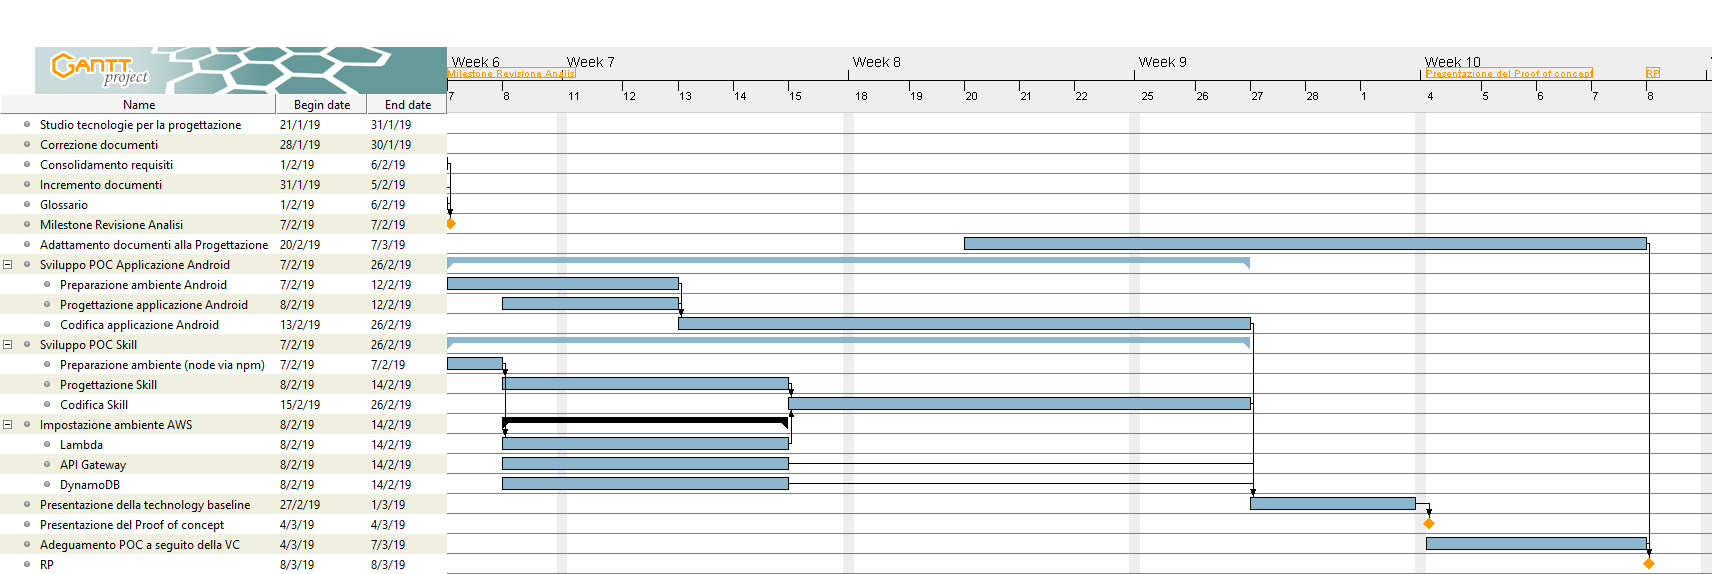
\includegraphics[scale=0.2]{./images/ZeroSevenGanttProgettazione.png}
    \caption{\textit{Diagramma di Gantt$_{G}$}: Base tecnologica }\label{G3}
\end{figure}
\newpage
\section{Progettazione di Dettaglio e Codifica}\label{PrDeC}
\textbf{Periodo:} da 2019-03-09 a 2019-04-12\\
Questo periodo inizia dopo la Revisione di Progettazione e termina  alla Revisione di Qualifica.\\
In questo periodo avviene la codifica vera e propria del prodotto finale.\\
Le attività della periodo di Progettazione di Dettaglio e Codifica sono:
\begin{itemize}
	\item \textbf{Correzione e incremento documenti}; 
	\item \textbf{Piano dei test di unità}: il gruppo progetta i test di unità, che vengono tracciati con i loro metodi; 
	\item \textbf{Sviluppo applicazione Android}: comprende la progettazione in dettaglio di ogni classe Android e la seguente codifica;
	\item \textbf{Sviluppo skill}: comprende la progettazione in dettaglio di ogni classe in nodeJS e la seguente codifica. Lo sviluppo deve avvenire seguendo i principi \textit{Test Driven Development$_{G}$}, come suggerito dalla proponente. Prima di sviluppare ogni metodo, è necessario fornire il relativo test di unità;
	\item \textbf{Sicurezza}: il gruppo studia ogni parte del sistema in sviluppo e implementa le best practice per assicurare la sicurezza di queste;
	\item \textbf{Manuali}: vengono redatti opportuni manuali del prodotto in fase di sviluppo, sia per l'utente che per lo sviluppatore;
	\item \textbf{Product Baseline}: viene presentata in modalità Agile la progettazione a livello di dettaglio, riportando diagrammi e contestualizzando le principali scelte architetturali adottate.
\end{itemize}
I ruoli maggiormente coinvolti sono: \textit{Responsabile}, \textit{Amministratore}, \textit{Progettista}, \textit{Verificatore} e \textit{Programmatore}.
\begin{figure} [h]
   
    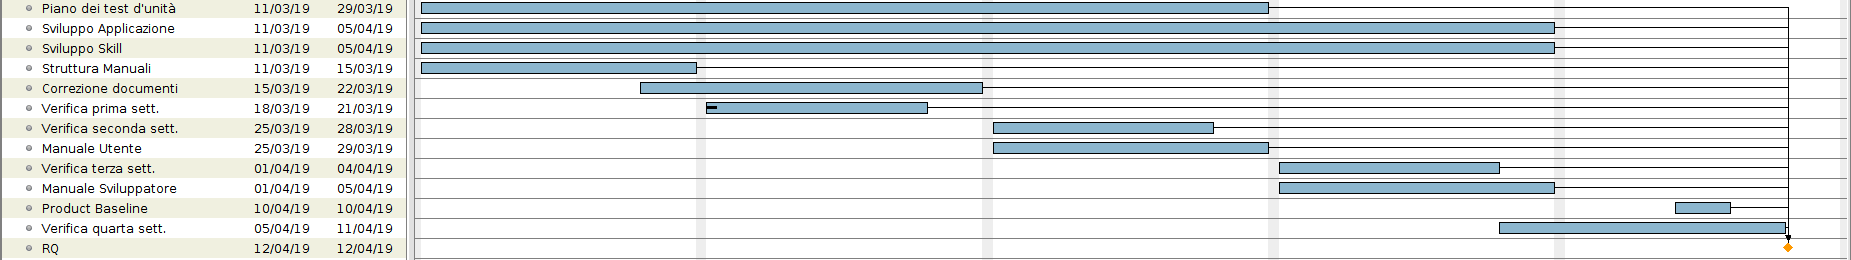
\includegraphics[scale=0.2]{./images/ZeroSevenGanttCodificaDettaglio.png}
    \caption{\textit{Diagramma di Gantt$_{G}$}: Progettazione di dettaglio e Codifica }\label{G4}
\end{figure}

Segue il dettaglio (suddiviso per settimane) delle attività da svolgere per ogni punto descritto alla sezione \ref{PrDeC}
\subsection{Da 2019-03-09 a 2019-03-15}\label{DCprimaSett}
\begin{itemize}
	
	\item \textbf{Piano dei test di unità:} codifica dei test di unità in modo da arrivare al 33\% di copertura per la skill.
	\item \textbf{Sviluppo applicazione Android:} codifica dei blocchi Sport, News e Crypto, progettazione del design pattern architetturale seguendo MVVM sfruttando i framework forniti da android, codifica completa della gerarchia di classi adibita alla comunicazione con API Gateway;
	\item \textbf{Sicurezza}: implementazione di OAuth per l'autenticazione di Alexa;
	\item \textbf{Manuali}: fornire una struttura di base per la scrittura dei manuali.
	
\end{itemize}


\subsection{Da 2019-03-16 a 2019-03-22}
\begin{itemize}
		
	\item \textbf{Correzione e incremento documenti:} aggiornamento dei documenti secondo le direttive ricevute in RP, compreso l'aggiornamento degli strumenti introdotti(TypeScript in particolare);
	\item \textbf{Verifica:} verifica di quanto prodotto nella settimana precedente;
	\item \textbf{Piano dei test di unità:} codifica dei test di unità in modo da arrivare al 66\% di copertura per la skill;
	\item \textbf{Sviluppo skill:} Codifica delle parti della struttura coperte da test, in particolare blocchi News Borsa, Crypto e Sport in modo da poter effettuare l'integrazione delle parti prodotte fin'ora.\\
	Stesura dei diagrammi di sequenza e attività da presentare alla Producti Baseline;
	\item \textbf{Sviluppo applicazione Android:} Codifica del blocco lista e pin, implementazione del design pattern architetturale, stesura dei diagrammi di sequenza e attività relativi alla rimozione di blocchi e workflow da presentare alla Product Baseline, insieme ai diagrammi delle classi relativi a Weather e Twitter.
\end{itemize}


\subsection{Da 2019-03-23 a 2019-03-29}
\begin{itemize}
	\item \textbf{Verifica:} verifica di quanto prodotto nella settimana precedente;
	\item \textbf{Piano dei test di unità:} codificare i test d'unità in modo da ottenere la copertura completa del codice
	\item \textbf{Sviluppo applicazione Android:} codifica dei blocchi progettati non ancora implementati (v. sezione \ref{DCprimaSett});
	\item \textbf{Sviluppo skill:} codifica del blocco Weather (coperto da test) e Twitter per quanto riguarda la lettura di hashtag e timeline di un utente;
	\item \textbf{Manuali:} stesura del manuale utente fino al suo completamento per la Revisione di Qualifica.  
\end{itemize}

\subsection{Da 2019-03-30 a 2019-04-06}
 	\item \textbf{Verifica:}verifica di quanto prodotto nella settimana precedente;
	\item \textbf{Sviluppo applicazione Android:} codifica dell'interfaccia grafica e integrazione fra le parti interne della app;
	\item \textbf{Sviluppo Skill:} codifica dei blocchi pin e lista(in lettura), seguendo la progettazione precedentemente prodotta;
	\item \textbf{Manuali:} stesura del manuale sviluppatore fino al suo completamento per la Revisione di Qualifica.
\subsection{Da 2019-04-07 a 2019-04-11}
	\item \textbf{Verifica:} Verifica di quanto prodotto nella settimana precedente;
	\item \textbf{Correzione e incremento documenti:} stesura dei preventivi e consuntivi a finire relativi al periodo, aggiornamento delle metriche nel \pianodiqualifica, attualizzazione dei rischi, a seguire approvazione per il rilascio di tutti i documenti per la Revisione di Qualifica;
	\item \textbf{Product Baseline:} presentazione di Product Baseline

\newpage
\section{Validazione e Collaudo}
\textbf{Periodo:} da 2019-04-12 a 2019-05-17\\
Questo periodo inizia al termine della Progettazione di Dettaglio e Codifica e si conclude con la Revisione di Accettazione.\\
Il prodotto è pronto e il team effettua dei test di verifica su di esso che ne precedono la validazione.\\
Le attività che svolge il gruppo sono:
\begin{itemize}
   \item \textbf{Maturità documenti}: vengono apportate le ultime modifiche ai documenti, secondo i risultati della RQ;
   \item \textbf{Validazione}: l'intero sistema viene validato rispetto ai requisiti coerentemente con i test di sistema individuati nel periodo di Analisi;
   \item \textbf{Consuntivo finale}: viene calcolato un consuntivo finale dell'intero progetto;
   \item \textbf{Manuali}: il manuale dell'utente viene completato;
   \item \textbf{Collaudo}: viene collaudo l'intero sistema, in presenza di Committente e Proponente, rispetto al capitolato e ai requisiti individuati. 
\end{itemize}
\begin{figure} [h]
    \centering
    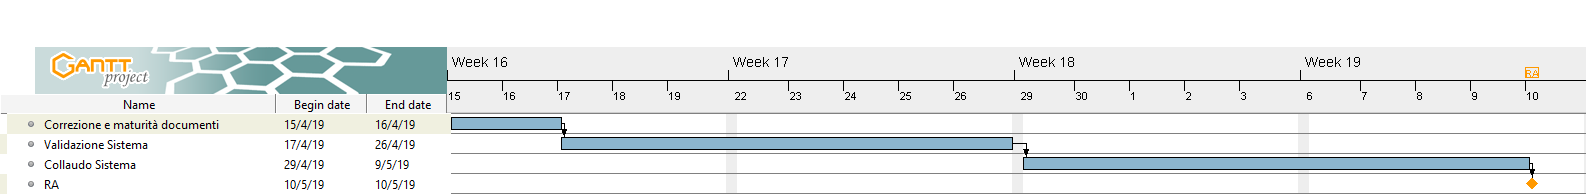
\includegraphics[scale=0.29]{./images/ZeroSevenGanttVerifica.png}
    \caption{\textit{Diagramma di Gantt$_{G}$}: Validazione e Collaudo }\label{G5}
\end{figure}
\end{flushleft}